\section*{Fouriertransformation Aufgaben mit L�sungen}\label{MA2-fouriertransformation-loesungen}

\ifintegriereaufgaben Erkl�rungen und Beispiele, die zum Verst�ndnis der L�sungswege hilfreich sind, finden Sie im Skript\wennreferenzvorhanden{MA2-fouriertransformation}{ (Abschnitt \abschnittsverweis{MA2-fouriertransformation})}. \fi



\begin{exercisebox}[Fourier-Transformation]
	Berechnen Sie die Fourier-Transformierte der folgenden Funktionen.
\begin{itemize}
	\item[(a)] $\delta > 0$
		\[ f:t\mapsto \begin{cases} e^{-\delta t}, \quad &t\geq 0\,,\\
				0\quad & t< 0\,.
			\end{cases}
		\]
	\item[(b)]
		\[ f:t\mapsto \begin{cases} \cos^2(t), \quad &|t| \leq \pi/2\,,\\
				0\quad & \textnormal{sonst}
			\end{cases}
		\]
	\item[(b)] $f: t\mapsto t\cdot e^{-|t|}$
\end{itemize}
\vspace{0.3cm}
\textbf{L�sung:} \newline

		Es kann hilfreich sein Symmetrieeigenschaften der Funktion zu untersuchen bevor man die Fourier-Transformierte berechnet, denn es gilt
	\begin{eqnarray*}
		\textnormal{gerade Funktionen}\; f(-t) &=& f(t) \Rightarrow \quad  \hat f(\omega) = \frac{2}{\sqrt{2\pi}} \int\limits_{0}^\infty f(t)\cdot \cos(\omega t)\,\mathrm{d}t\,,\\
		\textnormal{ungerade Funktionen}\; f(-t) &=& -f(t) \Rightarrow \quad \hat f(\omega) = \frac{-2i}{\sqrt{2\pi}} \int\limits_{0}^\infty f(t)\cdot \sin(\omega t)\,\mathrm{d}t\,.
	\end{eqnarray*}
	\begin{itemize}
			\item[(a)]
				\begin{eqnarray*}
					\hat f(\omega) &=& \frac{1}{\sqrt{2\pi}}\frac{\delta - i \omega}{\omega^2 + \delta^2} \\
						\Rightarrow |\hat f(\omega)| &=& \frac{1}{\sqrt{2\pi}}\frac{1}{\omega^2 + \delta^2} \quad \textnormal{Betrag}\,,\\
			\Rightarrow \varphi (\omega) &=& -\arctan\frac{\omega}{\delta} \quad \textnormal{Phase}\,.
		\end{eqnarray*}
	\item[(b)] Die Fouriertransformierte von \(f\) lautet:
		\[
		\hat f(\omega) = \frac{2}{\sqrt{2\pi}} \int\limits_{0}^{\pi/2} \cos^2(t) \cos(\omega t) \, \mathrm{d}t = \dfrac{4}{\sqrt{2\pi}} \dfrac{1}{\omega\,( 4 - \omega^2)} \sin\left(\omega \frac{\pi}{2}\right)\]
	Da $f$ eine gerade Funktion ist, l��t sich \(\hat f\) wie folgt berechnen \[ \hat f(\omega) = \dfrac{2}{\sqrt{2\pi}} \int\limits_0^\infty f(t) \cdot \cos(\omega\, t) \,\mathrm{d} t = \dfrac{2}{\sqrt{2\pi}} \int\limits_0^{\frac{\pi}{2}}  \cos^2(t) \cdot \cos(\omega\, t) \,\mathrm{d} t\,.\] Folgen wir dem Hinweis und schauen nach einem passenden Addtionstheorem zur Vereinfachung des Integranden. Es gilt
	\begin{equation}\label{additionstheorem} \cos^2( t ) = \dfrac12 \cdot \left( 1 + \cos(2\, t)\right) \,,\end{equation} und  damit
	\begin{equation}\label{ft} \hat f(\omega ) \stackrel{\eqref{additionstheorem}}{=} \dfrac{1}{\sqrt{2\pi}} \int\limits_0^{\frac{\pi}{2}}  \left(1 + \cos(2\,t)\right) \cdot \cos(\omega\, t) \,\mathrm{d} t  = \dfrac{1}{\sqrt{2\pi}}\left( \textcolor{red}{ \int\limits_0^{\frac{\pi}{2}}  \cos(\omega \, t) \,\mathrm{d} t} + \textcolor{blue}{\int\limits_0^{\frac{\pi}{2}} \cos(2\,t) \cdot \cos(\omega\, t) \,\mathrm{d} t} \right)  \,. \end{equation}
	Betrachten wir zu allererst den Fall \(\omega\not = 0\) und l�sen die beiden Integrale rechts getrennt. Das erste Integral rechts ist nicht schwer - es gilt:
	\[ \textcolor{red}{\int\limits_0^{\frac{\pi}{2}}  \cos(\omega \, t) \,\mathrm{d} t} = \left[ \dfrac{1}{\omega} \sin(\omega \, t ) \right]_0^{\frac\pi2} = \dfrac1\omega \sin\left( \omega \,\dfrac\pi2\right)\,.\]
	Zum L�sen des zweiten Integrals wenden wir zweimal eine partielle Integration an und das liefert:
	\begin{eqnarray*}
		&& \textcolor{blue}{\int\limits_0^{\frac{\pi}{2}} \cos(2\,t) \cdot \cos(\omega\, t) \,\mathrm{d} t}  \stackrel{ \mathrm{P.I.}}{=} \underbrace{ \left[ \cos(2\,t)\cdot \dfrac{1}{\omega} \sin(\omega\, t) \right]_0^{\frac{\pi}{2}}}_{-\dfrac{1}{\omega}\sin( \omega\, \frac\pi2)}  +\dfrac{2}{\omega} \int\limits_0^{\frac{\pi}{2}} \sin(2\,t)\cdot \sin(\omega\, t) \,\mathrm{d} t \\
		&\stackrel{ \mathrm{P.I.}}{=}&- \dfrac{1}{\omega}\sin( \omega\, \frac\pi2) + \dfrac2\omega \left(  \underbrace{ \left[ -\sin(2\,t)\cdot \dfrac1\omega\, \cos( \omega\,t)\right]_0^{\frac\pi2}}_{=0} + \dfrac{2}{\omega} \textcolor{blue}{ \int\limits_0^{\frac{\pi}{2}} \cos(2\,t) \cdot \cos(\omega\, t) \,\mathrm{d} t} \right)\\
		&=&- \dfrac{1}{\omega}\sin( \omega\, \frac\pi2) + \dfrac{4}{\omega^2} \textcolor{blue}{ \int\limits_0^{\frac{\pi}{2}} \cos(2\,t) \cdot \cos(\omega\, t) \,\mathrm{d} t}\,.
\end{eqnarray*}
Wir haben eine algebraische Gleichung erhalten, die sich nach unserem unbekannten Integral aufl�sen l��t!
\[ \Rightarrow \textcolor{blue}{\int\limits_0^{\frac{\pi}{2}} \cos(2\,t) \cdot \cos(\omega\, t) \,\mathrm{d} t} = - \dfrac{1}{ 1- \dfrac{4}{\omega^2} } \dfrac{1}{\omega} \, \sin\left( \omega \dfrac\pi2\right) = \dfrac{\omega}{4-\omega^2} \sin\left( \omega \dfrac\pi2\right) \,.  \]
Setzten wir die Integrale in \eqref{ft} ein, so erhalten wir f�r \(\omega \not = 0\)
\[ \hat f(\omega ) = \dfrac{1}{\sqrt{2\pi}} \dfrac1\omega \sin\left( \omega \,\dfrac\pi2\right) + \dfrac{\omega}{4-\omega^2} \sin\left( \omega \dfrac\pi2\right) =  \dfrac{1}{\sqrt{2\pi}} \dfrac{ 4}{\omega\,(4-\omega^2)} \sin\left( \omega \dfrac\pi2\right) \]
Betrachten wir jetzt  \(\omega=0\):
\[ \hat f(0) \stackrel{\eqref{additionstheorem}}{=} \dfrac{1}{\sqrt{2\pi}} \int\limits_0^{\frac\pi2} \left( 1 + \cos(2\,t)\right) \mathrm{d} t = \dfrac{1}{\sqrt{2\pi}}\cdot \dfrac{\pi}{2}  \]
Mit der Regel von L'Hospital ist
\[ \lim\limits_{\omega\to 0} \dfrac{\sin\left(\omega \dfrac{\pi}{2}\right)}{\omega} =  \dfrac{\pi}{2} \]
gilt f�r alle \(\omega \in \mathbb R\):
\[ \hat f(\omega ) = \dfrac{1}{\sqrt{2\pi}} \dfrac{ 4}{\omega\,(4-\omega^2)} \sin\left( \omega \dfrac\pi2\right) \]

	\item[(c)] $f$ ist eine ungerade Funktion
		\[
		\hat f(\omega) = \frac{-2i}{\sqrt{2\pi}} \int\limits_{0}^\infty te^{-t} \sin(\omega t) \, \mathrm{d}t = -\frac{1}{\sqrt{2\pi}}\frac{4i\omega}{\omega^4+ 2\omega^2 +1}\]

\end{itemize}
\end{exercisebox}

\begin{exercisebox}[Fourier-Transformation der Gau�schen Funktion]
	Bestimmen Sie die Fourier-Transformierte der Gau�schen Glockenkurve \( f: t \mapsto e^{-\frac{t^2}{2}} \). Benutzen Sie ohne Beweis die folgende Identit�t \( \int\limits_{-\infty}^\infty e^{-z^2}\mathrm{d} z = \sqrt{\pi}\) wobei  \(z\in \mathbb C\,.\)

\vspace{0.3cm}
\textbf{L�sung:} \newline
			\begin{eqnarray*}
				\hat f(\omega) &=& \frac{1}{\sqrt{2\pi}} \int\limits_{-\infty}^\infty e^{-\frac{t^2}{2}} e^{-i\omega t}\,\mathrm{d}t \stackrel{(*)}{=} \frac{1}{\sqrt{2\pi}} \int\limits_{-\infty}^\infty e^{-\frac12 (t+i\omega)^2} \cdot e^{-\frac12 \omega^2} \,\mathrm{d}t \\ &\stackrel{ (**)}{=}& \frac{2}{\sqrt{2\pi}} e^{-\frac12 \omega^2} \int\limits_{-\infty}^\infty e^{-z^2} \,\mathrm{d}z = \sqrt{2} e^{-\frac12 \omega^2}\,,
			\end{eqnarray*}
			wobei
			\begin{itemize}
				\item der Exponent in \( (*) \) durch die quadratische Erg�nzung umgeformt worden ist \[ -\frac12 t^2 - i\omega t = -\frac12\left( t^2 + 2i\omega t + (i\omega t)^2 \right) + \frac12 (i\omega)^2 = -\frac12\left( t+i\omega\right)^2 + \frac12(i\omega)^2 \,.\]
				\item das Integral durch die Substitution \( z = \frac12 (t+i\omega)\) in ein Integral �ber die komplexen Variable \(z\) �bergeht.
			\end{itemize}
Wichtig ist die Interpretation dieses Ergebnisses: Die Fourier-Transformierte einer Gau�schen Glockenkurve ist wieder die Gau�sche Glockenkurve!
\end{exercisebox}

\begin{exercisebox}[Fourier-Transformation]
	Im Skript wurde die Idee verfolgt die Fourier-Transformation mathematisch als Grenzprozess aus der Fourier-Reihe zu entwickeln. Den Grenzprozess schauen wir uns an einem konkreten Beispiel jetzt an.
\begin{itemize}
	\item[(a)] Zeigen Sie, dass gilt \[ c_{k} = \frac{\Delta \omega}{\sqrt{2\pi}} \cdot \tilde c_{k}, \quad \tilde c_{k} = \frac{1}{\sqrt{2\pi}} \cdot\int\limits_{-\frac{T}{2}}^{\frac{T}{2}} f(t)\cdot e^{-i\, \omega_k \,t} \,\mathrm{d} t, \quad \textnormal{mit Kreisfrequenz}\; \omega_k = \frac{2\pi k}{T}\,.\]
	\item[(b)] Betrachten Sie nun die $T$-periodische Funktion $f$ mit \( f|_{T}:[-T/2, T/2)\to \mathbb R,   t\mapsto e^{-|t|}\) und bestimmen Sie eine Formel f�r die Fourierkoeffizienten \(\tilde c_k\).
%\item[(c)] Zeigen Sie, dass gilt  \[ \tilde c_{k} = \sqrt{\frac{2}{\pi}}\left( 1- (-1)^k e^{-T/2}\right) \cdot \frac{1}{1+ \omega_k^2} \,.\]
	\item[(c)] Berechnen Sie die Fourier-Transformierte $\hat g$ von $g: \mathbb R \to \mathbb R, t\mapsto e^{-|t|}$.
	\item[(d)] Setzen Sie \(T=50\) und bestimmen Sie mit Hilfe einer Software die Punkte \( \left( \omega_k, \tilde c_k \right), \, 1\leq k \leq 50\). Erzeugen Sie ein Bild, das die Punkte und die den Graph von \(\hat g\) zeigt und interpretieren Sie das Ergebnis.
\end{itemize}

\vspace{0.3cm}
\textbf{L�sung:} \newline
\begin{itemize}
	\item[(a)]  \[ \Delta\omega= \frac{2\pi}{T}\; \Rightarrow \; c_k = \frac{1}{T} \, \int\limits_{-T/2}^{T/2} f(t) \cdot e^{-i\, \omega_k \,t}\,\mathrm{d}t = \frac{\Delta \omega}{2\pi} \textcolor{blue}{\int\limits_{-T/2}^{T/2}f(t) \cdot e^{-i \, \omega_k \, t}\,\mathrm{d}t}  =  \frac{\Delta \omega}{\sqrt{2\pi}} \cdot \textcolor{blue}{ \tilde c_k }\,.\]
	\item[(b)]
		\begin{eqnarray*}
			c_0 &=& \frac{1}{T} \int\limits_{-\frac{T}{2}}^{\frac{T}{2}} e^{-|t|} \, \mathrm{d} t = \frac{2}{T} \, \int\limits_{0}^{\frac{T}{2}} e^{-t} \,\mathrm{d}t = \frac2T \,\Big[ - e^{-t}\Big]_0^{\frac{T}{2}} = \frac2T\, \left( 1-e^{-\frac{T}{2}}\right)\\
			c_k &=& \frac{1}{T} \int\limits_{-\frac{T}{2}}^{\frac{T}{2}} e^{-|t|}\cdot e^{-i \, \omega_k \,t} \, \mathrm{d} t = \frac{1}{\sqrt{2\pi}} \frac{1}{1+\omega_k^2} \\[1ex]
			&=& \frac{\Delta \omega}{\sqrt{2\pi}} \, \frac{2}{\sqrt{2\pi}} \frac{1}{1+\omega_k^2} \left( 1-(-1)^k\, e^{-\frac{T}{2}}\right) \\[2ex]
			\Rightarrow  \; \tilde c_k &=& \frac{2}{\sqrt{2\pi}} \frac{1}{1+\omega_k^2} \left( 1-(-1)^k\, e^{-\frac{T}{2}}\right) \,.
		\end{eqnarray*}

	%	Die Funktion \(f\) ist gerade und damit gilt \begin{equation}\label{bn_gerades_Signal} b_n = 0, \quad n\geq 1\,. \end{equation} Die Koeffizienten \(a_n\) lauten:
	%	\begin{eqnarray*}
	%		a_0 &=& \frac{2}{T} \int\limits_{-\frac{T}{2}}^{\frac{T}{2}} e^{-|t|} \,\mathrm{d}t = \frac{4}{T} \int\limits_{0}^{\frac{T}{2}} e^{-t} \,\mathrm{d}t = \frac4T \Big[ - e^{-t}\Big]_0^{\frac{T}{2}} = \frac4T\left( 1-e^{-\frac{T}{2}}\right) \,,\\
	%		a_n &=& \frac{2}{T} \int\limits_{-\frac{T}{2}}^{\frac{T}{2}} e^{-|t|} \cdot \cos\left( \frac{2\pi n t}{T}\right) \,\mathrm{d}t =\frac{4}{T} \int\limits_{0}^{\frac{T}{2}} e^{-t} \cdot \cos\left(\frac{2\pi n t}{T}\right) \,\mathrm{d}t \\  &\stackrel{(*)}{ = }& \frac4T \left(  \Big[ -\cos\left(\frac{2\pi n t}{T}\right) e^{-t}\Big]_0^{\frac{T}{2}} + \frac{2\pi n}{T} \Big[ \sin\left(\frac{2\pi n t}{T}\right) e^{-t}\Big]_0^{\frac{T}{2}} - \left( \frac{2\pi n }{T}\right)^2  \int\limits_0^{\frac{T}{2}} \cos\left(\frac{2\pi n t}{T}\right) e^{-t}\,\mathrm{d}t \right) \\
	%		&\stackrel{(**)}{=}& \frac{4}{T} \frac{1}{1+\left( \frac{2\pi n}{T}\right)^2} \left( 1-(-1)^ne^{-\frac{T}{2}}\right)  = \frac{4 }{T} \frac{1}{1+\omega_n^2} \left( 1-(-1)^ne^{-\frac{T}{2}}\right)\,.
	%					\end{eqnarray*}
	%					wobei in \( (*) \) zweimal partiell integriert und in \( (**)\) die Identit�t \( \cos(\pi n ) = (-1)^n\) ausgenutzt worden ist.
	\item[(c)] \begin{eqnarray*} \hat g(\omega) &=& \frac{1}{\sqrt{2\pi}} \int\limits_{-\infty}^\infty  e^{-|t|}\cdot e^{-i\, \omega\, t}\,\mathrm{d}t = \frac{1}{\sqrt{2\pi}} \left( \int\limits_{-\infty}^0 e^t \cdot e^{-i\, \omega\, t}\,\mathrm{d}t + \int\limits_{0}^\infty e^{-t} \cdot e^{-i\,\omega\, t}\,\mathrm{d}t\right) \\
			&=& \frac{1}{\sqrt{2\pi}} \left( \Big[ \frac{1}{1-i\,\omega} e^{(1-i\,\omega)\,t}\Big]_{-\infty}^0 + \Big[ -\frac{1}{1+i\,\omega} e^{-(1+i\,\omega)t}\Big]_0^\infty\right) \\
			&=& \frac{1}{\sqrt{2\pi}} \left( \frac{1}{1-i\,\omega} + \frac{1}{1+i\,\omega} \right) = \frac{1}{\sqrt{2\pi}} \left(  \frac{1+i\,\omega}{1+\omega^2}  + \frac{1-i\,\omega }{1+\omega^2} \right) \\
								&=& \frac{2}{\sqrt{2\pi}} \frac{1}{1+\omega^2}\,.
						\end{eqnarray*}
	%		Es gilt \[ \begin{cases} c_{k} &= \frac12 \cdot \left( a_k - i \, b_k\right)\,, \\ c_{-k} &= \frac12\cdot \left(a_k + i\, b_k\right)\end{cases} \quad \stackrel{\displaystyle{ \eqref{bn_gerades_Signal}}}{\Rightarrow}  \quad  \begin{cases} c_{k} &= \frac12\cdot a_k\,, \\ c_{-k} &= \frac12\cdot a_k\,. \end{cases} \]
	%					Mit \(T= \dfrac{ 2\pi}{ \Delta \omega}\) erhalten wir
	%					\begin{eqnarray*}
	%					c_{k} = c_{-k} &=& \frac12 \frac{4}{T} \frac{1}{1+\omega_k^2} \left( 1-(-1)^k \, e^{-\frac{T}{2}}\right) = \frac{2\,\Delta \omega}{2\pi}  \frac{1}{1+\omega_k^2} \left( 1-(-1)^k\, e^{-\frac{T}{2}}\right) \\ &=&  \frac{\Delta \omega}{\sqrt{2\pi}} \underbrace{ \frac{2}{\sqrt{2\pi}} \frac{1}{1+\omega_k^2} \left( 1-(-1)^k\, e^{-\frac{T}{2}}\right)}_{\displaystyle{=: \tilde c_k}} \,.  \end{eqnarray*}
					\item[(d)] Bild erzeugt mit Geogebra:
						\vspace{0.2cm}
						\begin{center}
							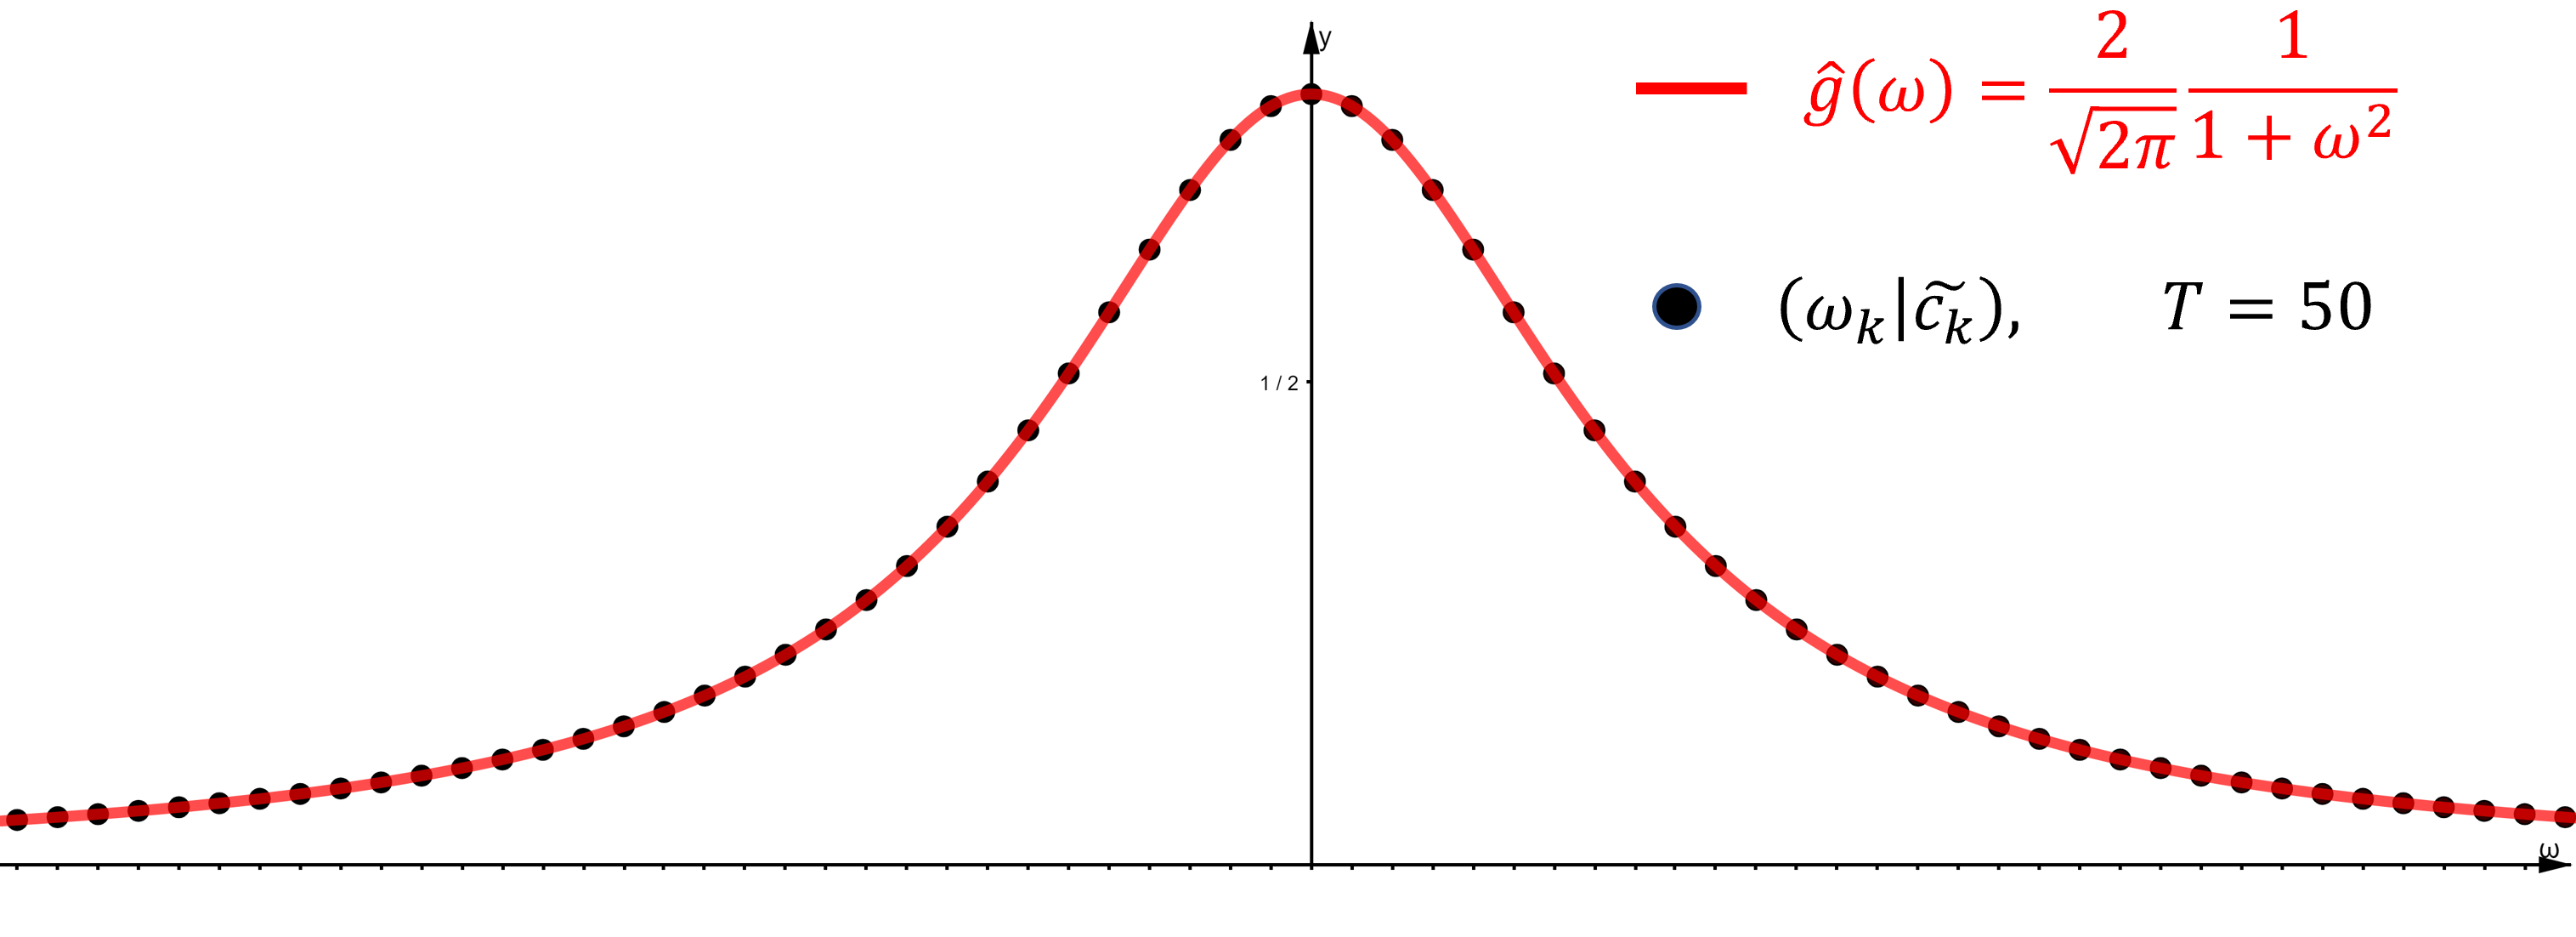
\includegraphics[width=0.8\textwidth]{../Mathematik_2/Bilder/fouriertransformation_grenzuebergang_von_fourierkoeffizienten.png}
			\end{center}
		\item[(e)] Das Spektrum von \(f\) sind diskrete Punkte im Frequenzraum \(\left( \omega_k \,|\, \tilde c_k\right) \, k \in \mathbb Z\). Die Punkte liege auf dem Graphen von \(\hat g\) und das sieht man auch analytisch: \[\lim\limits_{T\to \infty} \tilde c_k = \lim\limits_{T\to \infty}\frac{2}{\sqrt{2\pi}} \frac{1}{1+\omega_k^2} \left( 1-(-1)^k\, e^{-\frac{T}{2}}\right)  = \frac{1}{1+\omega_k^2} =  g(\omega_k) \,.\] Wichtig: der Grenz�bergang wird bez�glich der Variable \(T\) unternommen und zwar f�r eine fixierte Diskretisierung in \(\omega\)!
	\end{itemize}
\end{exercisebox}
%\begin{exercisebox}[Diskrete Fourier-Transformation]
%	Nehmen wir an das kontinuierlich gegebene Signal
%	\[ f: t\mapsto 5 + 2\cos(2\pi t - \pi/2) + 3\cos(4\pi t) \]
%	wird pro Sekunde vier Mal abgetastet.
%	\begin{itemize}
%		\item[(a)] Bestimmen Sie die Samples, die in einer Sekunde gemessen werden.
%		\item[(b)] Bestimmen Sie die diskrete Fourier-Transformation und zeigen Sie, dass sich die diskrete Fourier-Transformation als Matrix-Vektor-Multiplikation schreiben l��t.
%		\item[(c)] Wie l��t sich das Ergebnis interpretieren?
%	\end{itemize}
%\vspace{0.3cm}
%\textbf{L�sung:} \newline
%\begin{itemize}
%\item[(a)] F�r $S_l=(t_l, f(t_l))$ gilt $S_1 = \left(0,8\right), S_2= \left(\frac14,4\right), S_3=\left( \frac12, 8\right), S_4=\left( \frac34,0\right)$
%\item[(b)] Es gilt $\hat c_l = \displaystyle{ \sum\limits_{k=0}^3 e^{-i \,l\, \frac{2\pi}{N}  k} \cdot f(t_l) }$. Im vorliegenden Fall ist \(N=4\) und damit
%	\begin{eqnarray*}
%		\hat c_l = \displaystyle{ \sum\limits_{k=0}^3 e^{- i\,l \frac{2 \pi}{4} l} \cdot f(t_l) } \Rightarrow \left( \begin{array}{c} \hat c_0 \\\hat c_1 \\\hat c_2 \\ \hat c_3 \end{array}\right) = \left( \begin{array}{cccc} 1 & 1 & 1 & 1 \\ 1 & -i & -1 & i \\1 & -1 & 1 & -1 \\ 1 & i & -1 & -i \end{array}\right) \left( \begin{array}{c} 8 \\ 4 \\ 8 \\0\end{array}\right) \Rightarrow    \left( \begin{array}{c} \hat c_0 \\\hat c_1 \\\hat c_2 \\ \hat c_3 \end{array}\right) =\left( \begin{array}{c} 20 \\ -4i \\ 12  \\ 4i \end{array}\right)
%	\end{eqnarray*}
%\item[(c)] Die DFT liefert bis auf einen Skalierungsfaktor die Zerlegungskoeffizienten der harmonischen Schwingungen, die im Signal $f$ detektiert werden! Aus der DFT lassen sich die Samples zur�ckgewinnen durch die inverse, diskrete Fourier-Transformation (iDFT):
%	\[ f_k = \frac{1}{N}\sum\limits_{n=0}^{N-1} \hat c_n e^{i\, k\, \frac{2\pi}{N} n}\,. \]
%\end{itemize}
%\end{exercisebox}


